\chapter{A Wider View: Models of Other Supernova Remnants}\label{chp:chp6}

%\begin{flushright}
%  {\em QUOTE GOES HERE }\\
%
%\ \
%
%\normalsize
%{AUTHOR}  
%\end{flushright}


\noindent{FIRST PARAGRAPH}

\section{Introduction}
\section{SN~1980K}

\subsection{Smooth Models}
\begin{figure}
\centering
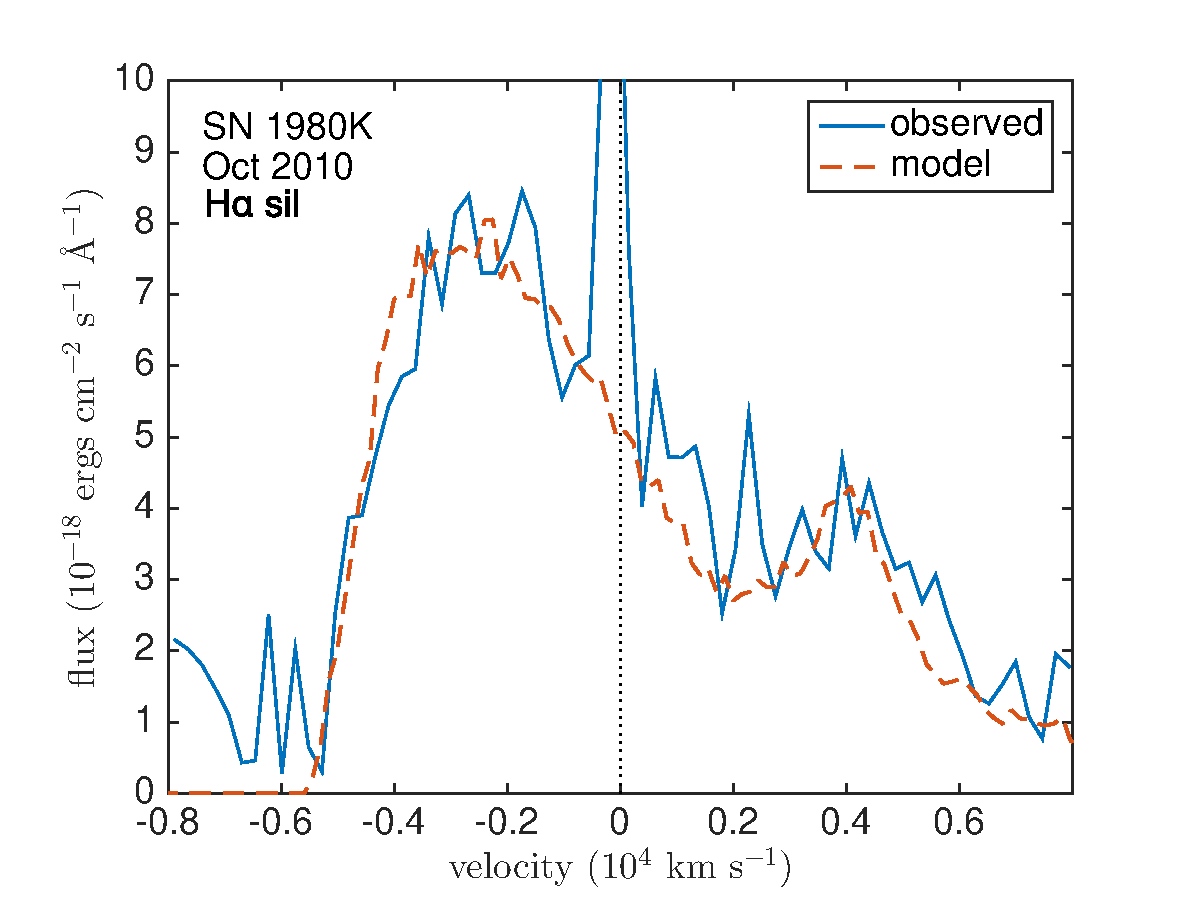
\includegraphics[scale=0.4,clip=true, trim=20 0 40 20]{chapters/chapter6/figs/80K/smooth/Ha}
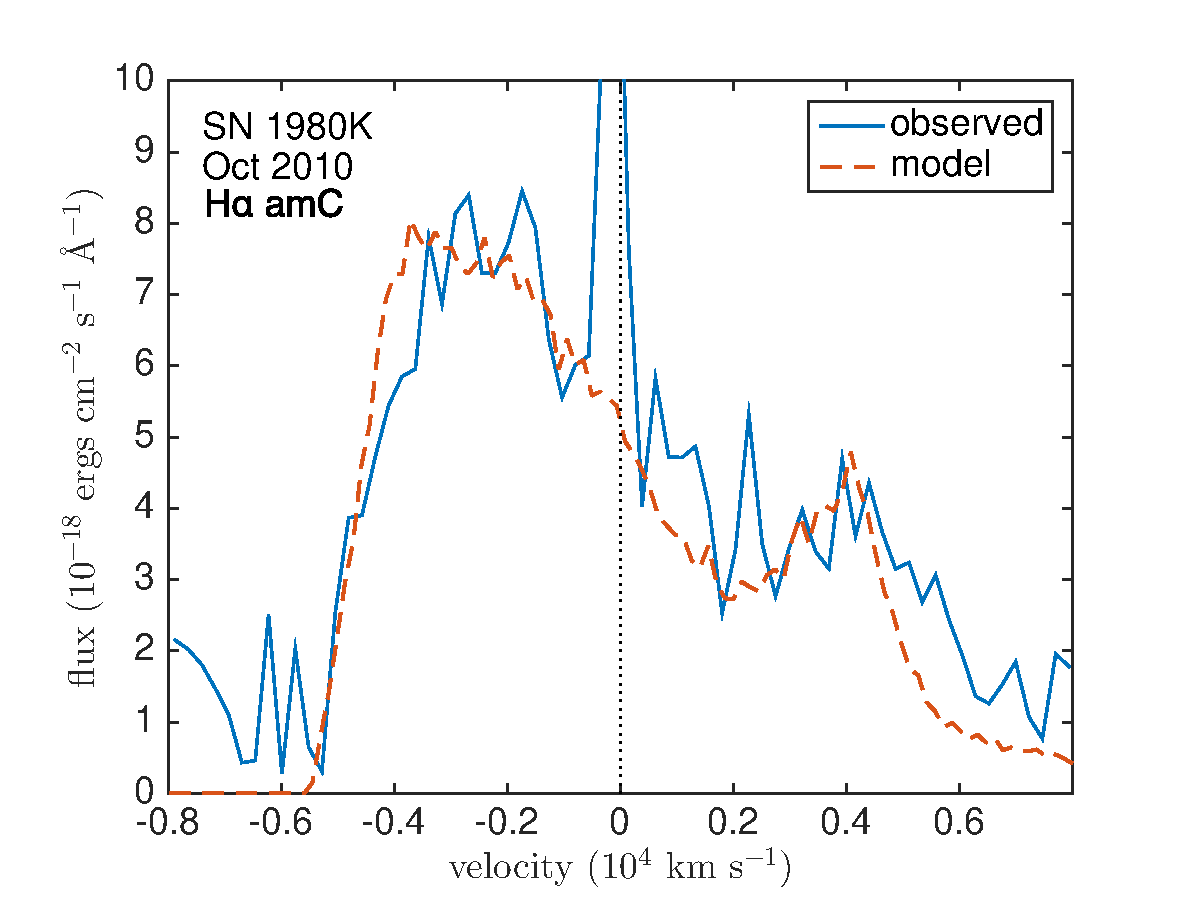
\includegraphics[scale=0.4,clip=true, trim=20 0 40 20]{chapters/chapter6/figs/80K/smooth/Ha_amC}

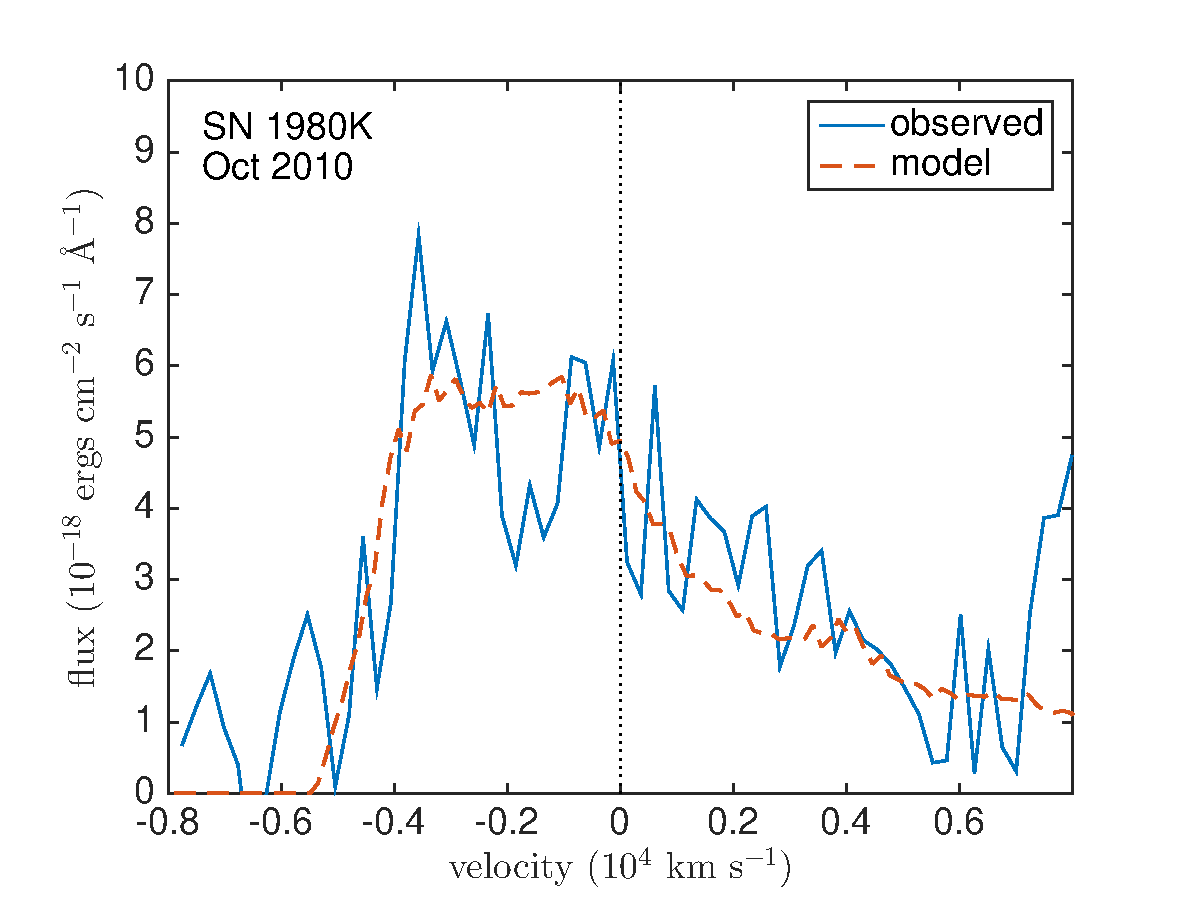
\includegraphics[scale=0.4,clip=true, trim=20 0 40 20]{chapters/chapter6/figs/80K/smooth/OI}
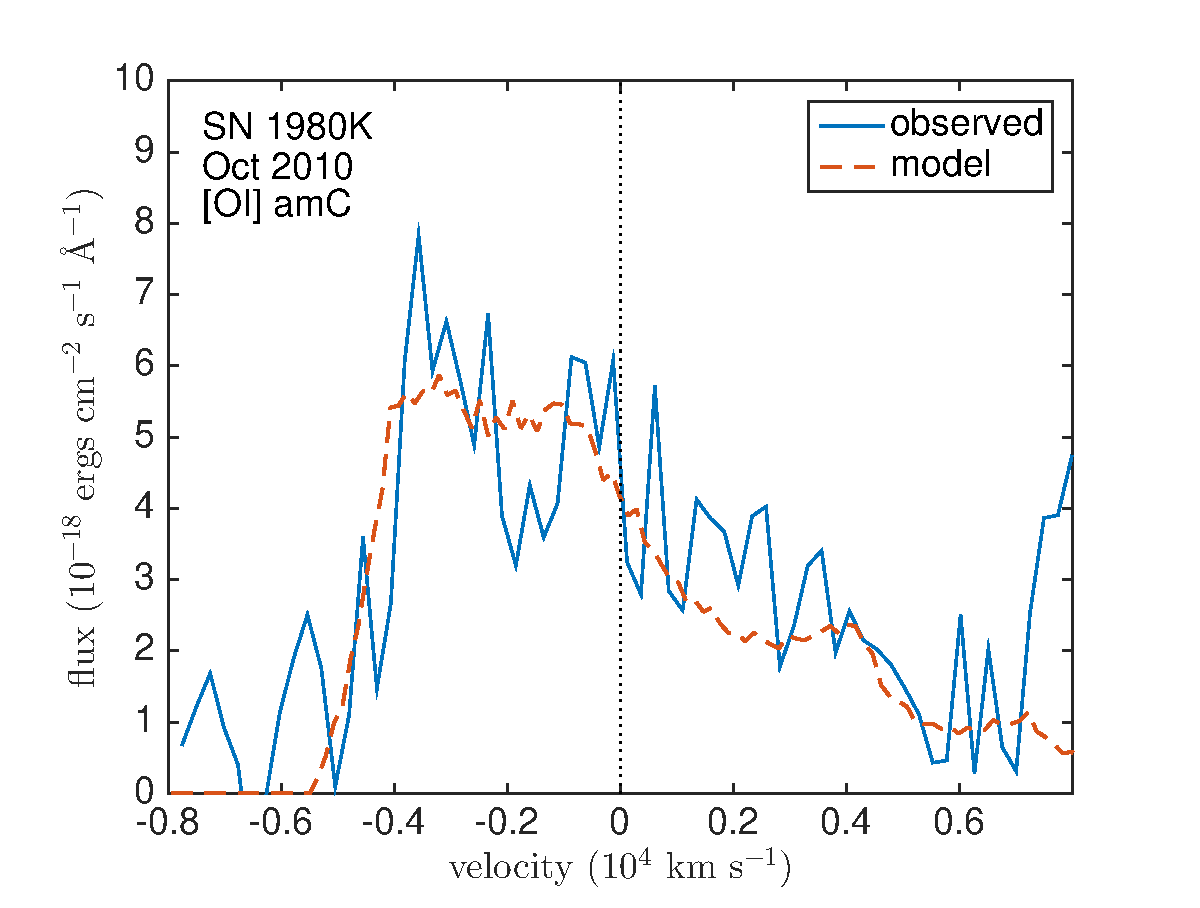
\includegraphics[scale=0.4,clip=true, trim=20 0 40 20]{chapters/chapter6/figs/80K/smooth/OI_amC}
\caption{Smooth fits to SN 1980K}
\label{80K_smooth}
\end{figure}

\begin{figure}
\centering
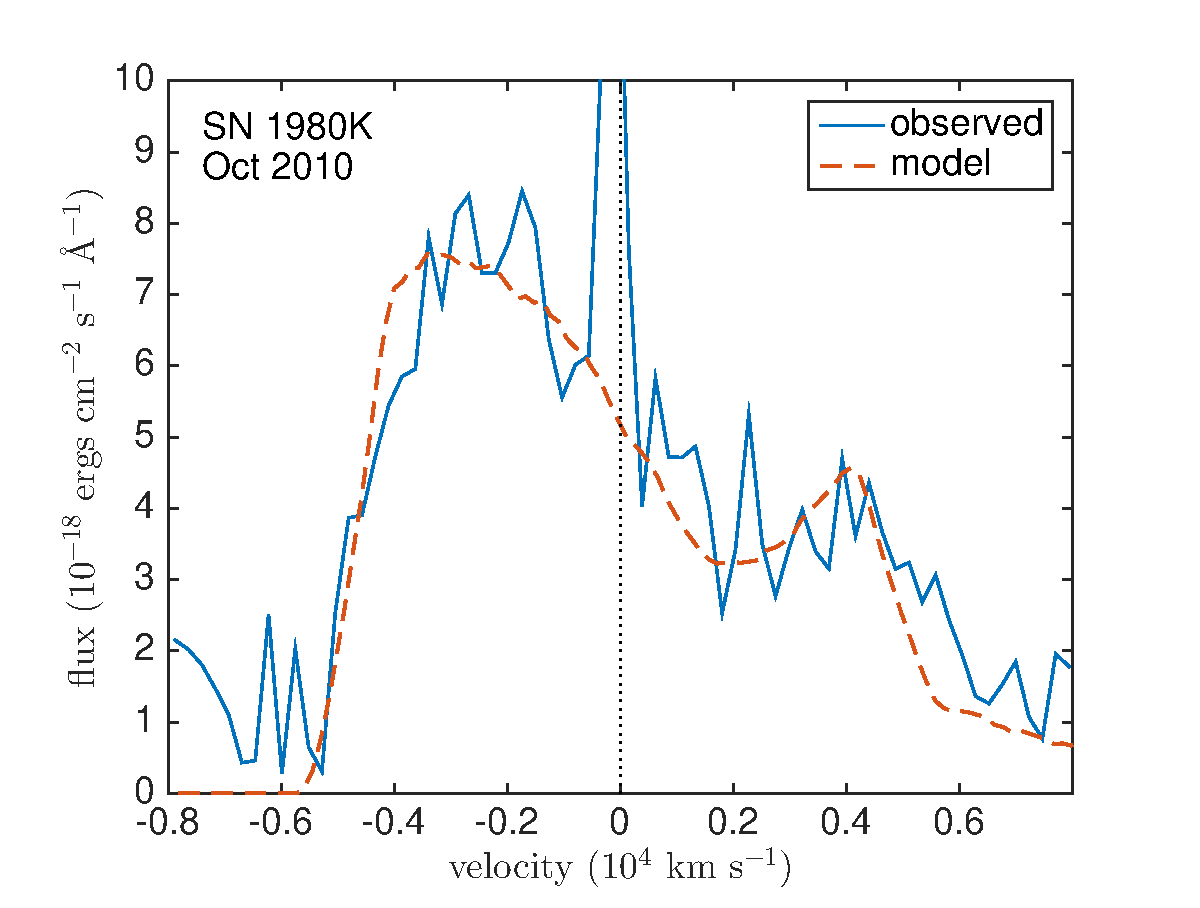
\includegraphics[scale=0.4,clip=true, trim=20 0 40 20]{chapters/chapter6/figs/80K/clumped/Ha}
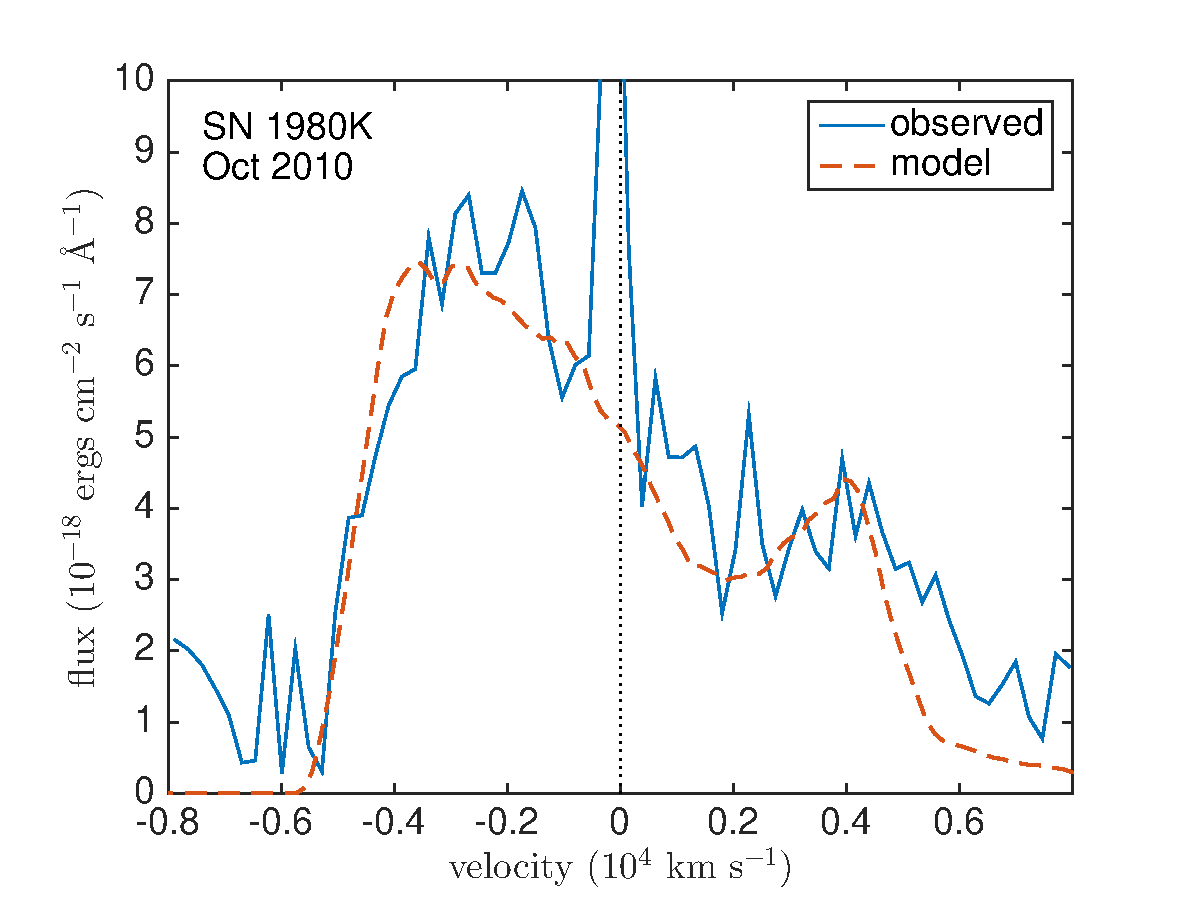
\includegraphics[scale=0.4,clip=true, trim=20 0 40 20]{chapters/chapter6/figs/80K/clumped/Ha_amC}

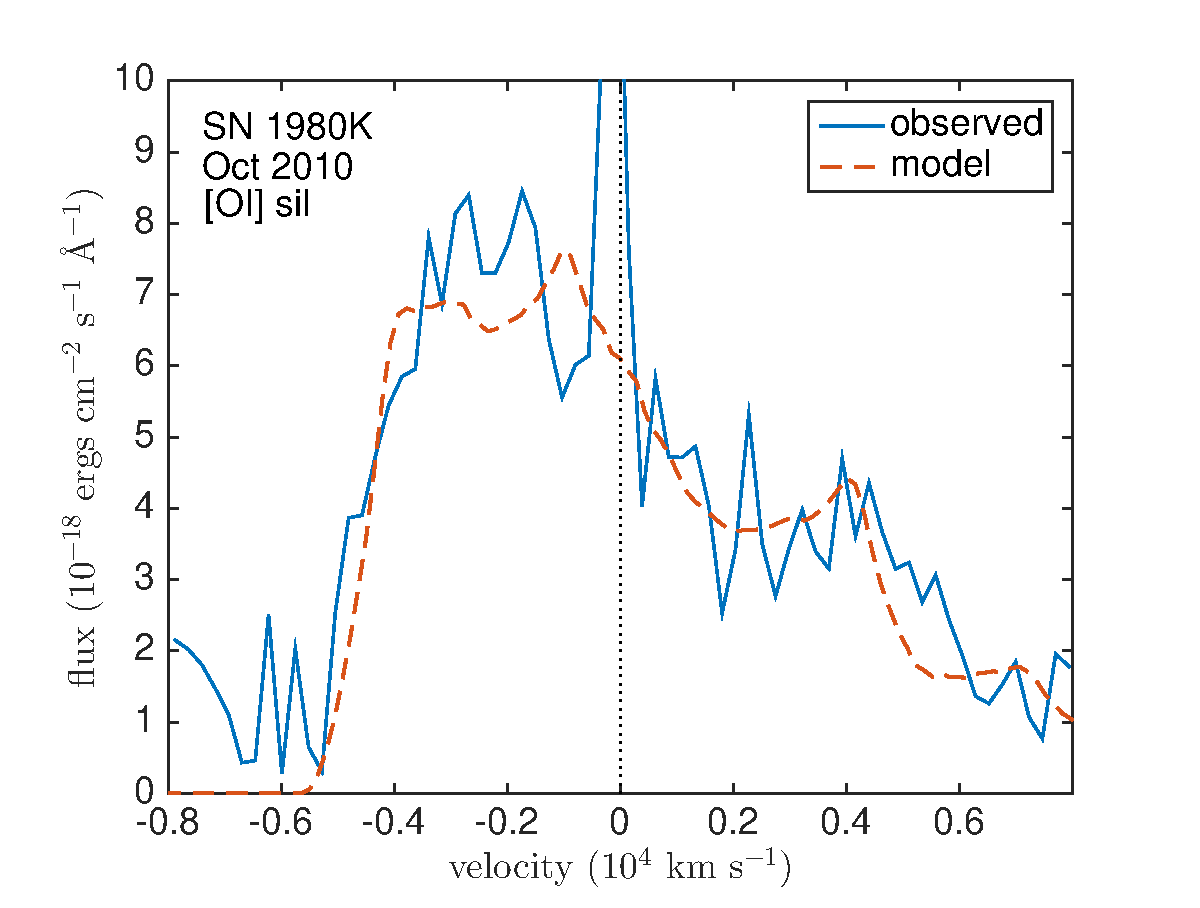
\includegraphics[scale=0.4,clip=true, trim=20 0 40 20]{chapters/chapter6/figs/80K/clumped/OI}
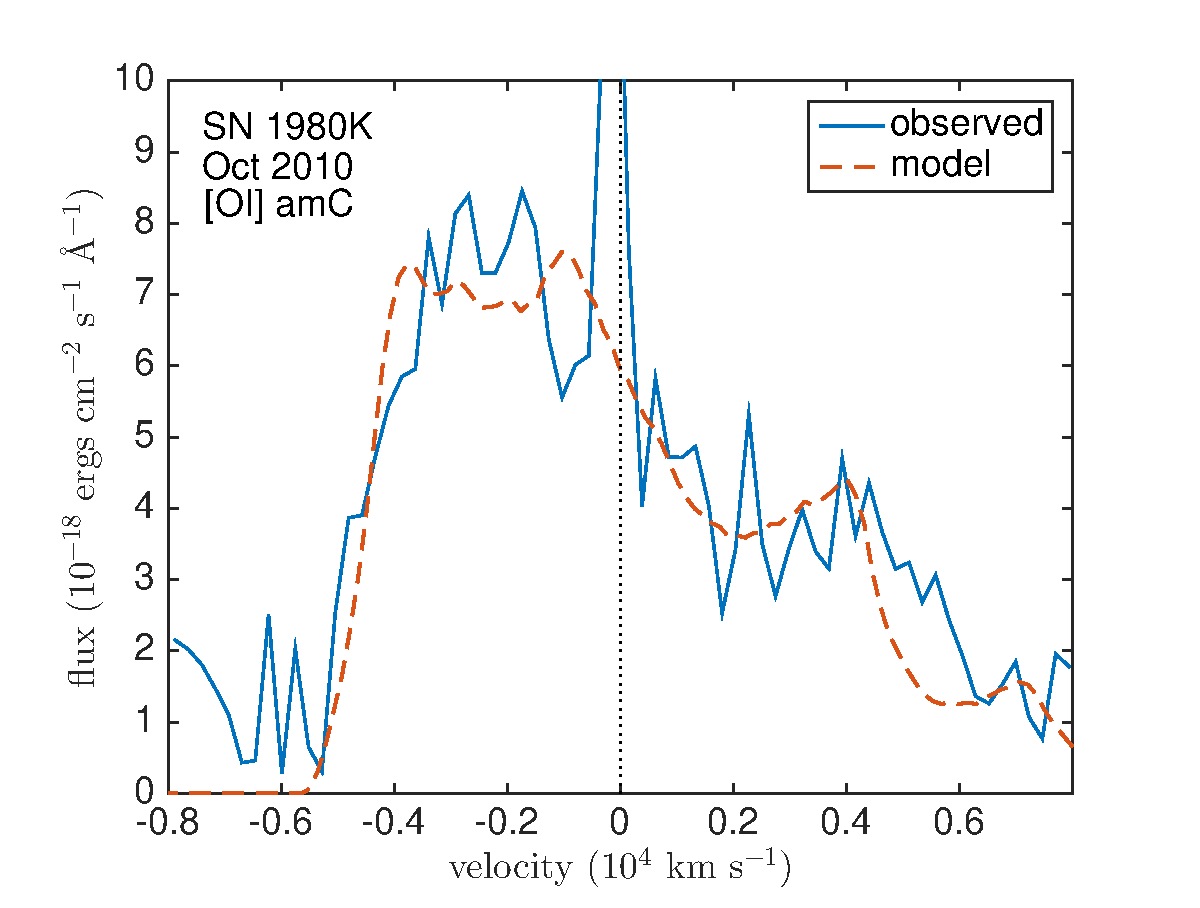
\includegraphics[scale=0.4,clip=true, trim=20 0 40 20]{chapters/chapter6/figs/80K/clumped/OI_amC}
\caption{clumped fits to SN 1980K}
\label{80K_clumped}
\end{figure}


\section{SN~1993J}
\begin{figure}
\centering
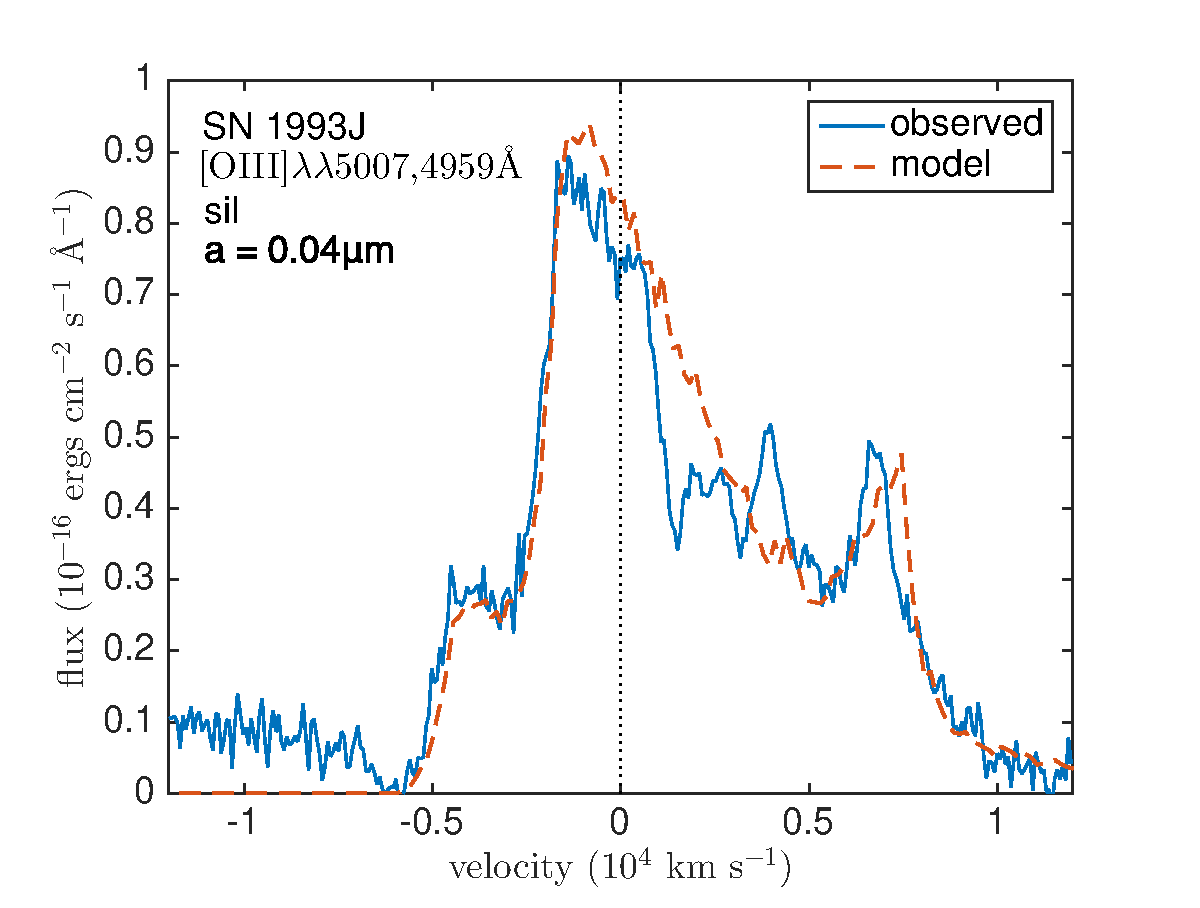
\includegraphics[scale=0.4,clip=true, trim=20 0 40 20]{chapters/chapter6/figs/93J/smooth/OIII}
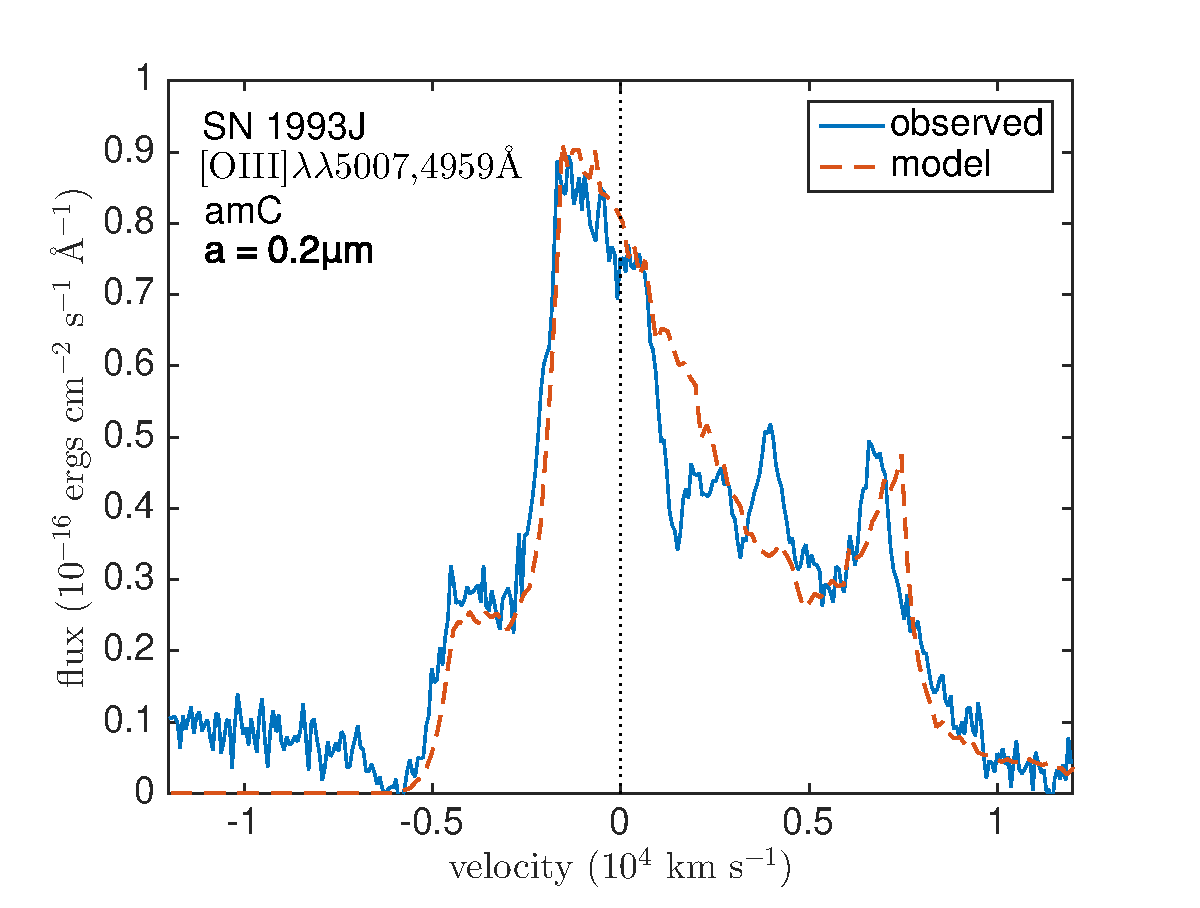
\includegraphics[scale=0.4,clip=true, trim=20 0 40 20]{chapters/chapter6/figs/93J/smooth/OIII_amC}

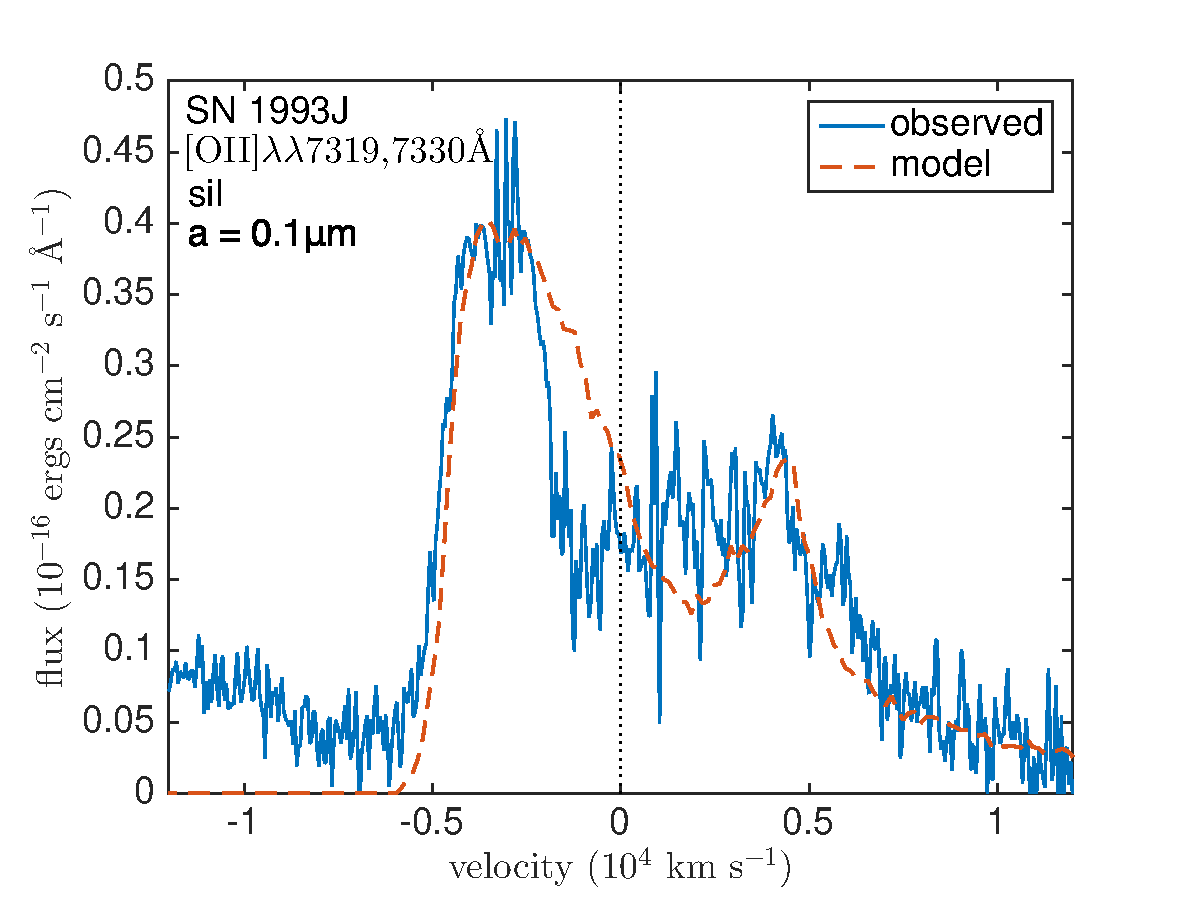
\includegraphics[scale=0.4,clip=true, trim=20 0 40 20]{chapters/chapter6/figs/93J/smooth/OII}
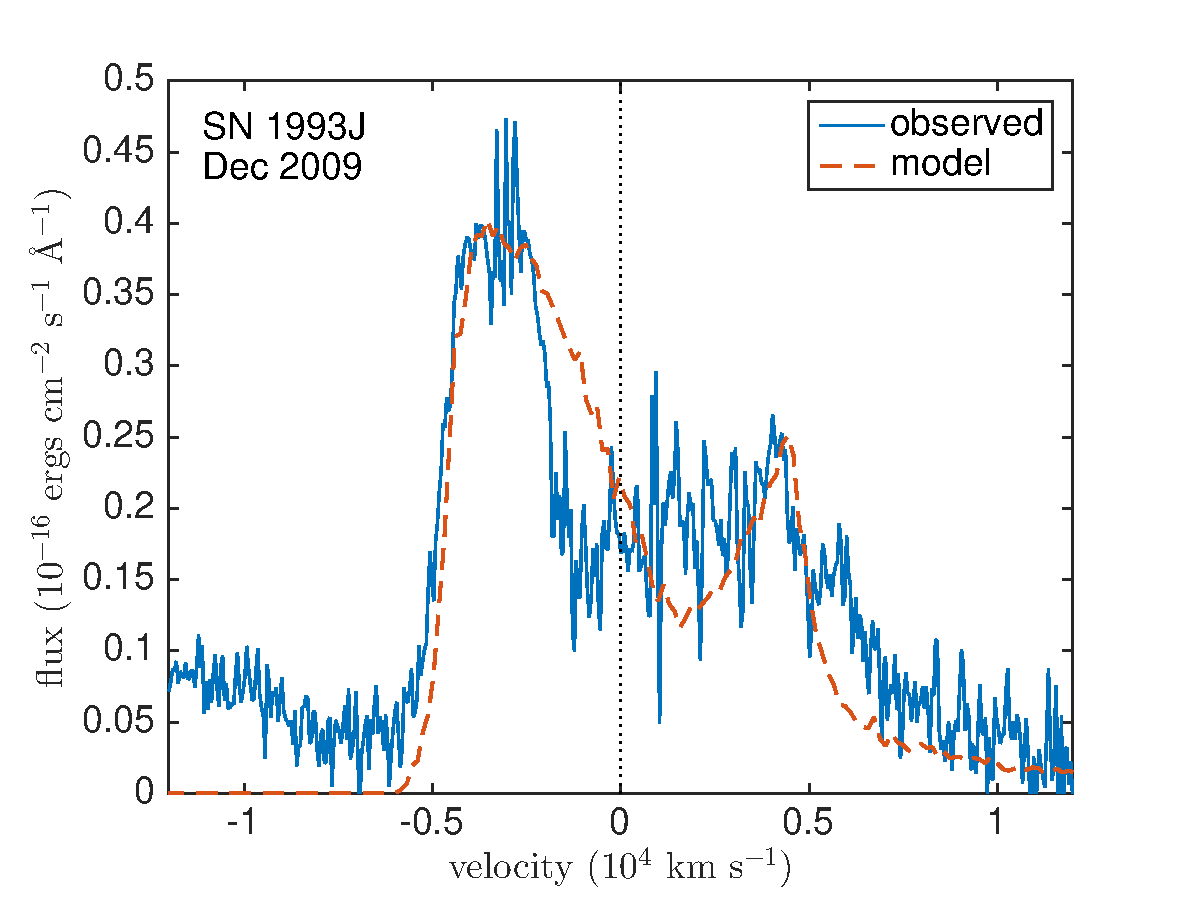
\includegraphics[scale=0.4,clip=true, trim=20 0 40 20]{chapters/chapter6/figs/93J/smooth/OII_amC}
\caption{smooth fits to SN 1993J}
\label{93J_smooth}
\end{figure}

\section{Cassiopeia A}

\subsection{Smooth Models}

Modelling was intially focussed on the OIII line, which exhibits a pronounced asymmetry.  Initial attempts to model this line produced a reasonable fit to the data.  The parameters used for this fit are detailed in Table \ref{} and the profile is presented in Figure \ref{}.  As can be seen, the fit fails to fit the red side of the profile well.  A manual investigation of parameter space resulted in the conclusion that the profile was much better fitted if the entire observed profile was shifted to the blue by $-700$ km s$^{-1}$.  This is not unexpected.  The integrated spectrum does sample the entire ejecta.  Additionally, Cas A is known to be significantly asymmetrical \citep{} and the integrated profile may well therefore have been initially shifted as a result of a net asymmetry in the line-of-sight velocities of the emitting regions.  This was also found to be the case with the OII line.  Throughout the remainder of my modelling I therefore allowed the profiles to be shifted to better fit the data.  Fits to the line profiles were significantly improved following this translation (see Figures \ref{} to \ref{}).

A model of the shifted OIII line is presented in Figure \ref{} and the parameters used for   this model are presented in Table \ref{}.  The line profile was shifted by $-700$ km s$^{-1}$.  An optical depth of $\tau=$ was found to best fit the profile.  A line profile model of the OIII line profile from Cas A could not be found using 100\% silicate dust (Draine).  There is little to no scattering wing seen and theerefore relativley small siliacte grains are required to reproduce the red side of hte profile.  Silicate grains of thi magnitude have extremely low absoprtion efficiencies and therefore The best-fitting optical depth of $\tau=$ corresponds to an implausibly large mass of dust )($>20$M$_{\odot}$ if it is composed entirely of astronomical siliactes \citep{Draine1984}.

The chemical composition of the dust in the eject of Cas A is known to be extremely complex.  There are many different species of dust grain present, and it is known that silicate dust is present based on features in teh spectrum.  However, the presence of a variety of other species is also predicted.  I therefore investigate the dust masses required to fit the profile for varying fractions of silicate and amorphous carbon dust.  In Table \ref{}, I detail the dust masses required to fit the OIII line profile for different fractions of silicates and carbon grains for a single grain size.  For each composition I determine the grain radius based on the albedo necessary to fit the profile.  The dust masses cover a wide range of values, although all are significantly higher than recent predictions based on Spitzer data by \citep{}.  

It might be possible for certain grain radii or wavelength to be able to determine the composition based on the wavelength dependence of the absorbing dust i.e. by considering anther blue-shifted line profile, we might be able to determine the composition based on the relative optical depths necessary to fit each line.  I therefore considered fitting the blue-shifted OII line from Cas A.  Sadly, at these grain sizes, there is not significant variation in the absoprtion efficiencies of either amorphous carbon or astronomilcal silicates between 5007\AA\ and 7319\AA and I therefore constrain the dust mass via this mechanism.  Additionally, the OII line is much less sensitive to variations in both distribution and dust mass.  However, I present a best fit to this line (shifted in this case by $-1000$ km s$^{-1}$) in Figure \ref{}  and detail the best-fitting parameters for this smooth case in Table \ref{}. 

I then consider the dust distribution and dust mass I derive for my best-fitting model to the OIII line profile and model this dust distribution with the emissivity distribution for the best-fitting OII model.  The resultant OII profile is a good fit and an improved fit over the original case when dust and gas were coupled.  This suggests that the two models are consistent and, if the relative abundance of species may be determined, that the dust masses are well-constrained.

\subsection{Clumped Models of Cas A}

The ejecta of Cas is highly clumped.  Recently, models by {Cherchneff paper} have suggested that dust cannot in fact form in the gas phase in the ejecta of Cas A unless extremely dense knots of material are present.  It is important to consider the effects of clumping on the line profiles.  I continue


\begin{figure}
\centering
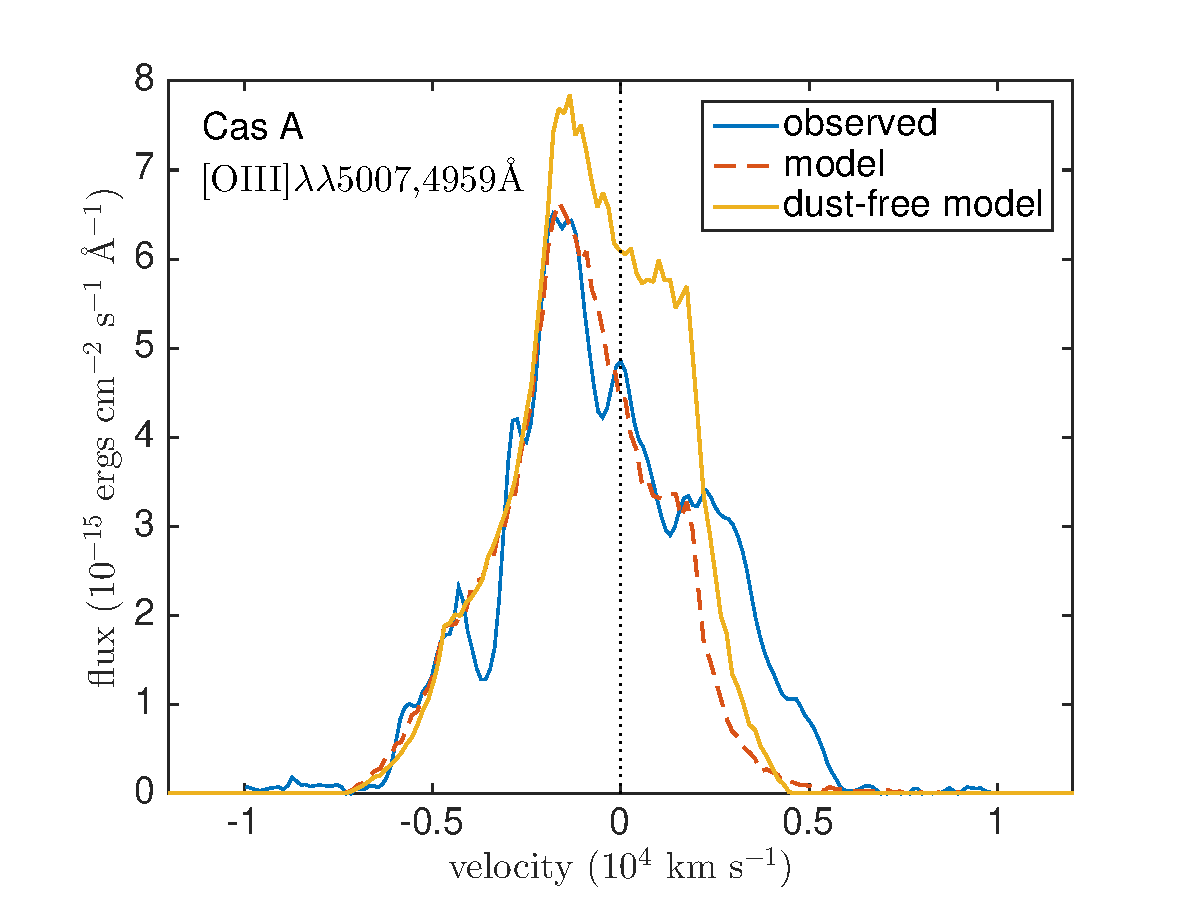
\includegraphics[scale=0.4,clip=true, trim=20 0 40 20]{chapters/chapter6/figs/CasA/CasA_OIII}
\caption{smooth fits to Cas A}
\label{CasA}
\end{figure}

\subsection{Clumped Models}



\subsection{Velocity-Shifted Line Profile Models}

\begin{figure}
\centering
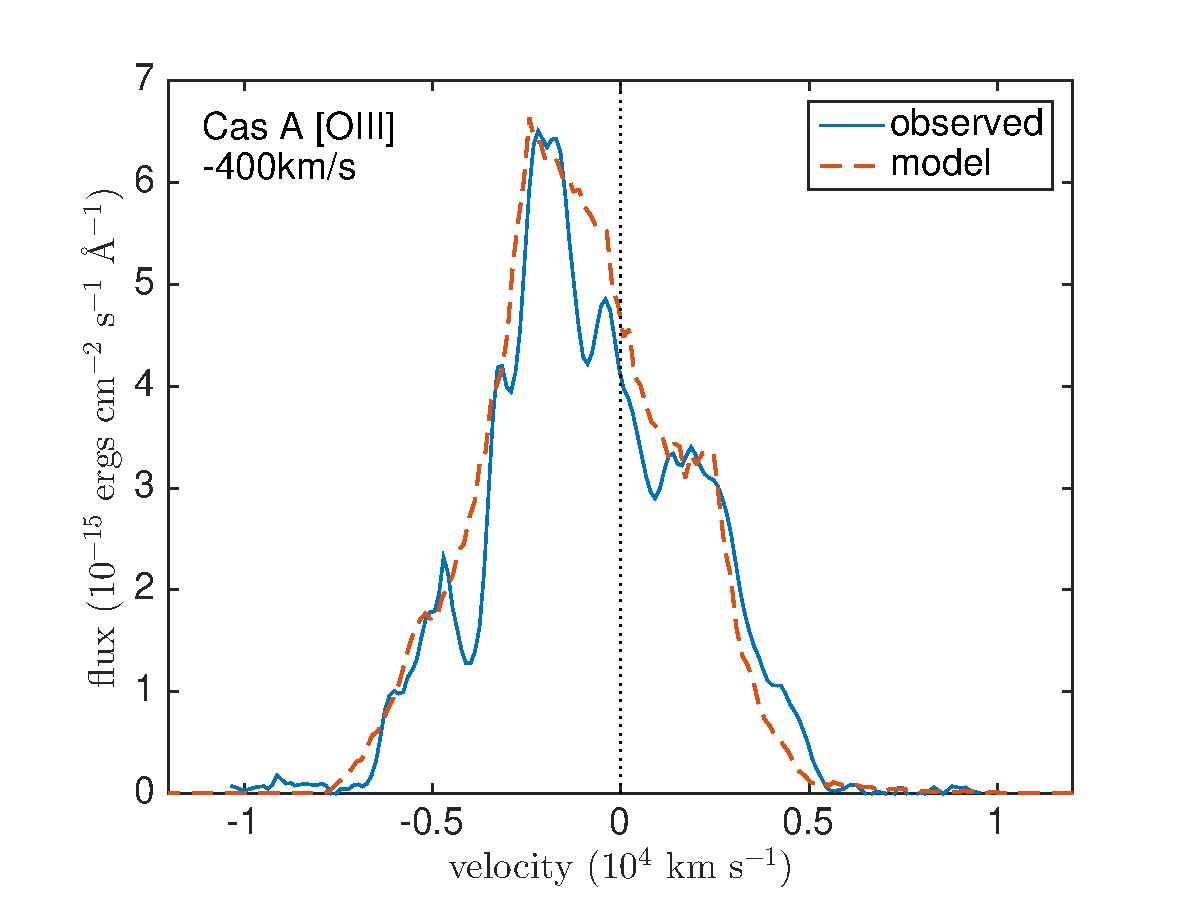
\includegraphics[scale=0.4,clip=true, trim=20 0 40 20]{chapters/chapter6/figs/CasA/CasA_OIII_v400shift}
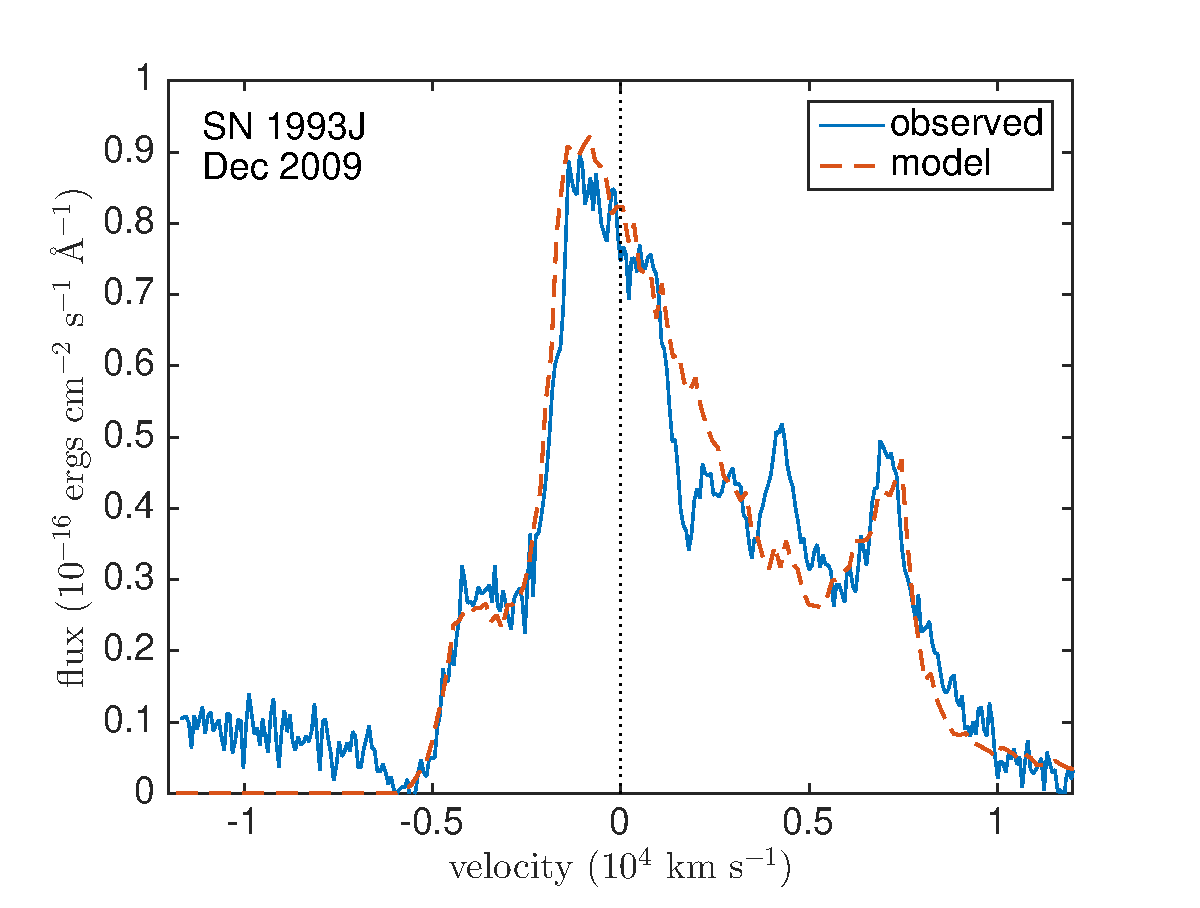
\includegraphics[scale=0.4,clip=true, trim=20 0 40 20]{chapters/chapter6/figs/93J/smooth/OIII_shifted_0_3}
\caption{shifted profiles of SN~1993J and Cas A}
\label{shifted}
\end{figure}

\begin{figure}
\centering
\fbox{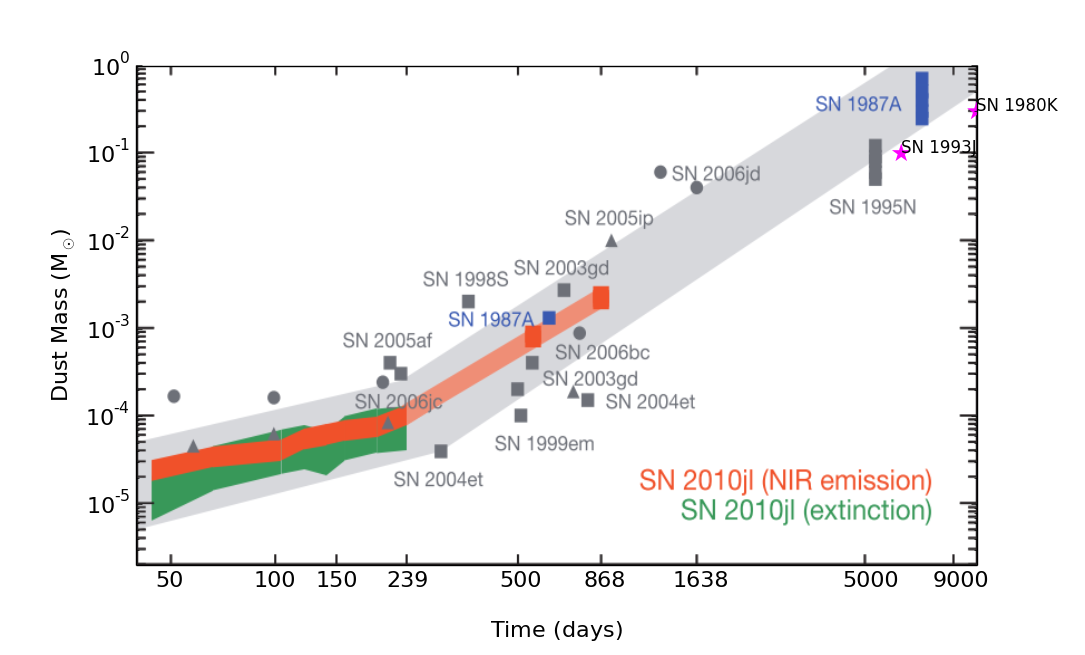
\includegraphics[scale=0.6,clip=true, trim=30 0 0 0]{chapters/chapter6/figs/test.png}}
\caption{dust masses}
\label{shifted}
\end{figure}


\section{Discussion}
\section{Conclusions}
